\begin{figure}
    \centering
    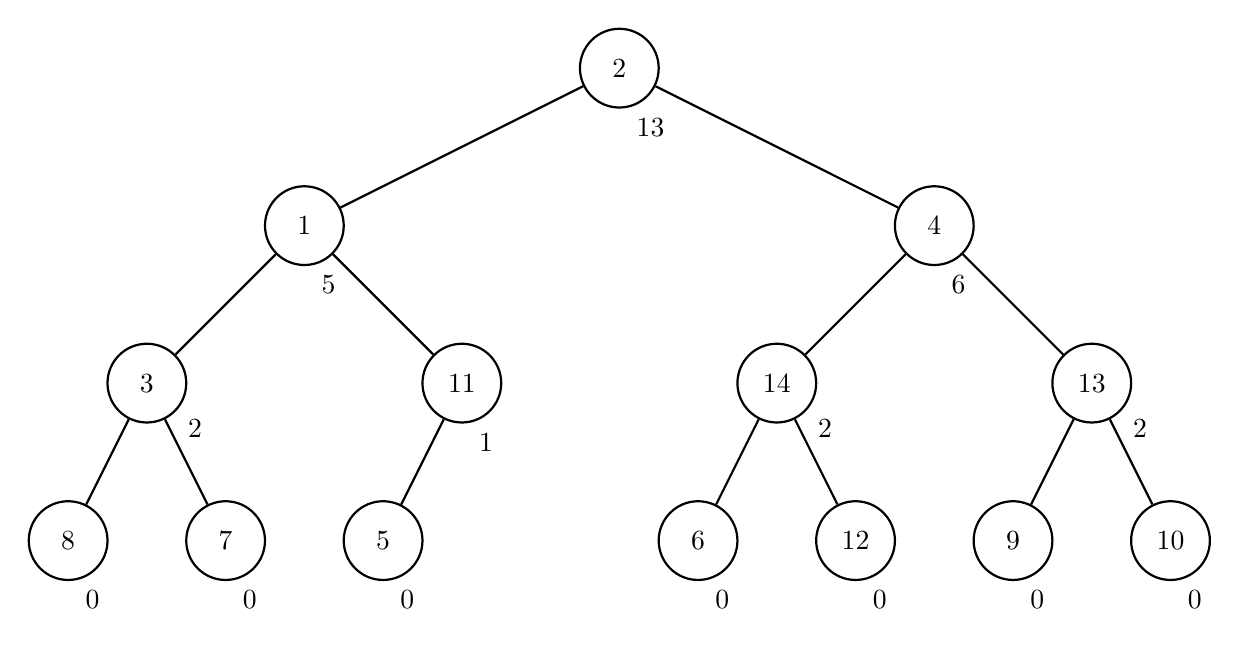
\begin{tikzpicture}[thick]
        \node[label=280:{13},circle,draw,minimum size=1cm]
            (1) at (0,0) {$2$};
        \node[label=280:{5},circle,draw,minimum size=1cm]
            (2) at (-4,-2) {$1$};
        \node[label=280:{6},circle,draw,minimum size=1cm]
            (3) at (4,-2) {$4$};
        \node[label=320:{2},circle,draw,minimum size=1cm]
            (4) at (-6,-4) {$3$};
        \node[label=280:{1},circle,draw,minimum size=1cm]
            (5) at (-2,-4) {$11$};
        \node[label=320:{2},circle,draw,minimum size=1cm]
            (6) at (2,-4) {$14$};
        \node[label=320:{2},circle,draw,minimum size=1cm]
            (7) at (6,-4) {$13$};
        \node[label=280:{0},circle,draw,minimum size=1cm]
            (8) at (-7,-6) {$8$};
        \node[label=280:{0},circle,draw,minimum size=1cm]
            (9) at (-5,-6) {$7$};
        \node[label=280:{0},circle,draw,minimum size=1cm]
            (10) at (-3,-6) {$5$};
        % \node[label={11},circle,draw,minimum size=1cm] (11) at (-1,-6) {$3$};
        \node[label=280:{0},circle,draw,minimum size=1cm]
            (12) at (1,-6) {$6$};
        \node[label=280:{0},circle,draw,minimum size=1cm]
            (13) at (3,-6) {$12$};
        \node[label=280:{0},circle,draw,minimum size=1cm]
            (14) at (5,-6) {$9$};
        \node[label=280:{0},circle,draw,minimum size=1cm]
            (15) at (7,-6) {$10$};

        \draw[thick] (1) -- (2);
        \draw[thick] (2) -- (4);
        \draw[thick] (4) -- (8);
        \draw[thick] (4) -- (9);
        \draw[thick] (2) -- (5);
        \draw[thick] (5) -- (10);
        % \draw[thick] (5) -- (11);
        \draw[thick] (1) -- (3);
        \draw[thick] (3) -- (6);
        \draw[thick] (3) -- (7);
        \draw[thick] (6) -- (12);
        \draw[thick] (6) -- (13);
        \draw[thick] (7) -- (14);
        \draw[thick] (7) -- (15);
    \end{tikzpicture}
    \caption[Como buscar $i$-ésimo na ABB]{Se quiséssemos encontrar
            o $7^\circ$ elemento na árvore acima, $i = 7$, desviamos
            para a direita, pois a quantidade de nós da subárvore
            direita da raiz é $\leq i$. Depois, desviamos para a
            esquerda e redefinimos $i$ como $3$, pois existem $4$
            elementos à frente. Como o nó do elemento $14$ só tem um
            nó em sua subárvore direita, desviamos para a esquerda
            de novo e redefinimos $i$ como $1$. Como a quantidade de
            nós da subárvore direita do nó do elemento $6$  somada a
            $1$ é igual a $i$, o elemento $6$ é o $7^\circ$ elemento
            da coleção.}
    \label{fig:abb:query}
\end{figure}